\section{Results}
\label{sec:results}

This is the results section.

\textcolor{red}{The results can be found in `figures/results`. This includes both figures
and tables for lookup of numbers and summary tables}


\begin{figure}[ht]
    \centering
    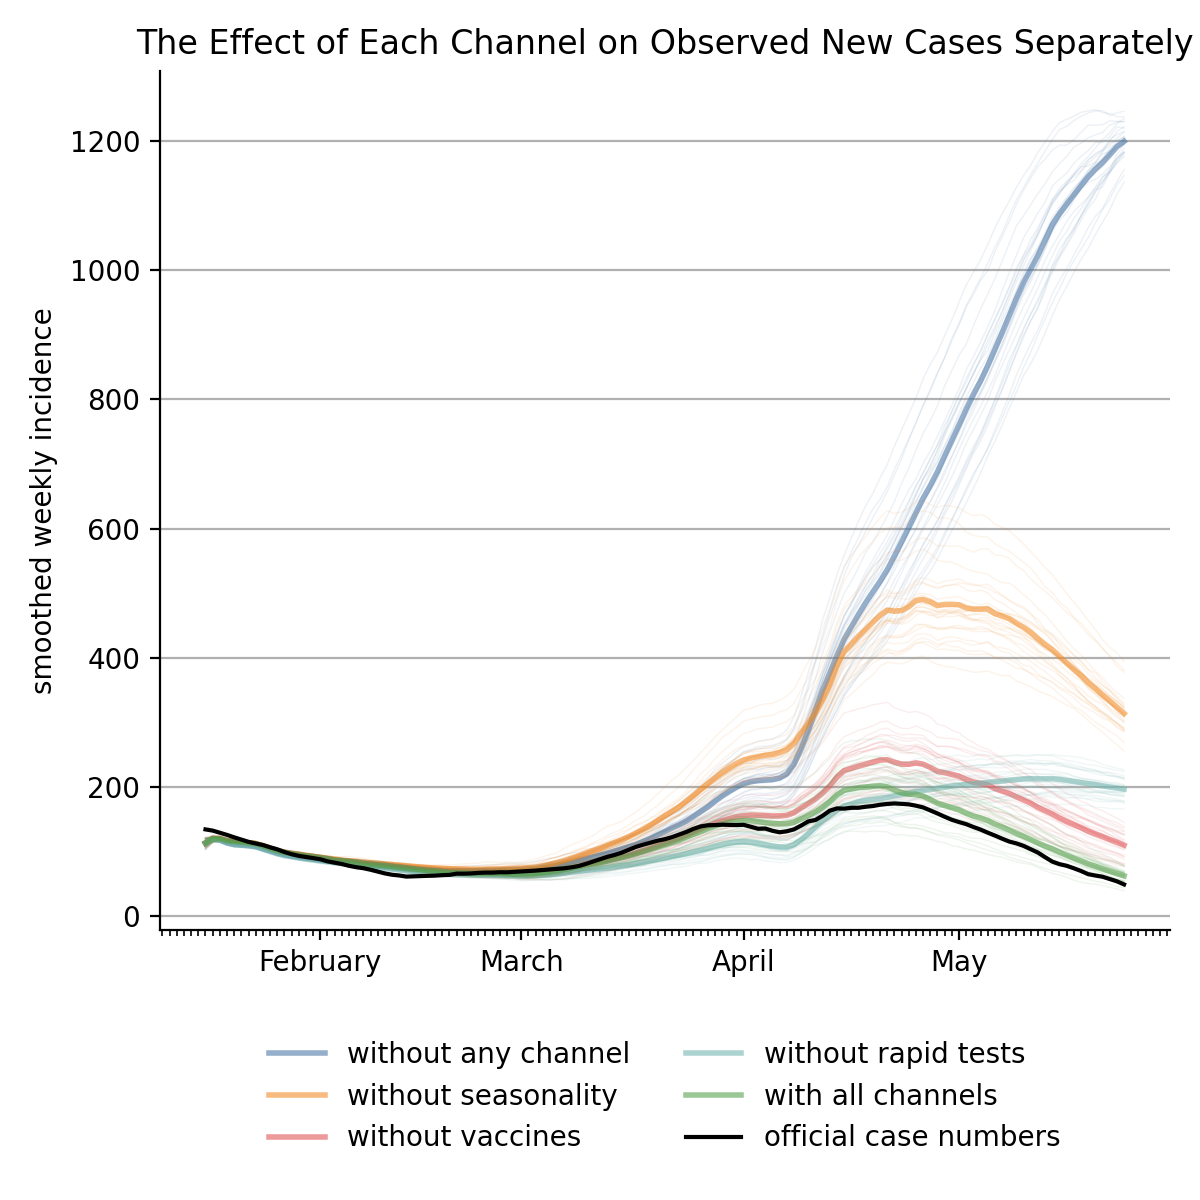
\includegraphics[width=0.9 \textwidth]{../figures/results/figures/comparisons/one_off_and_combined/full_new_known_case}
    \caption{The Effect of Each Channel on Observed New Cases Separately}
    \label{fig:explain_decline}
    \figurenotes{\textcolor{red}{\ldots}}
\end{figure}

\begin{figure}[ht]
    \centering
    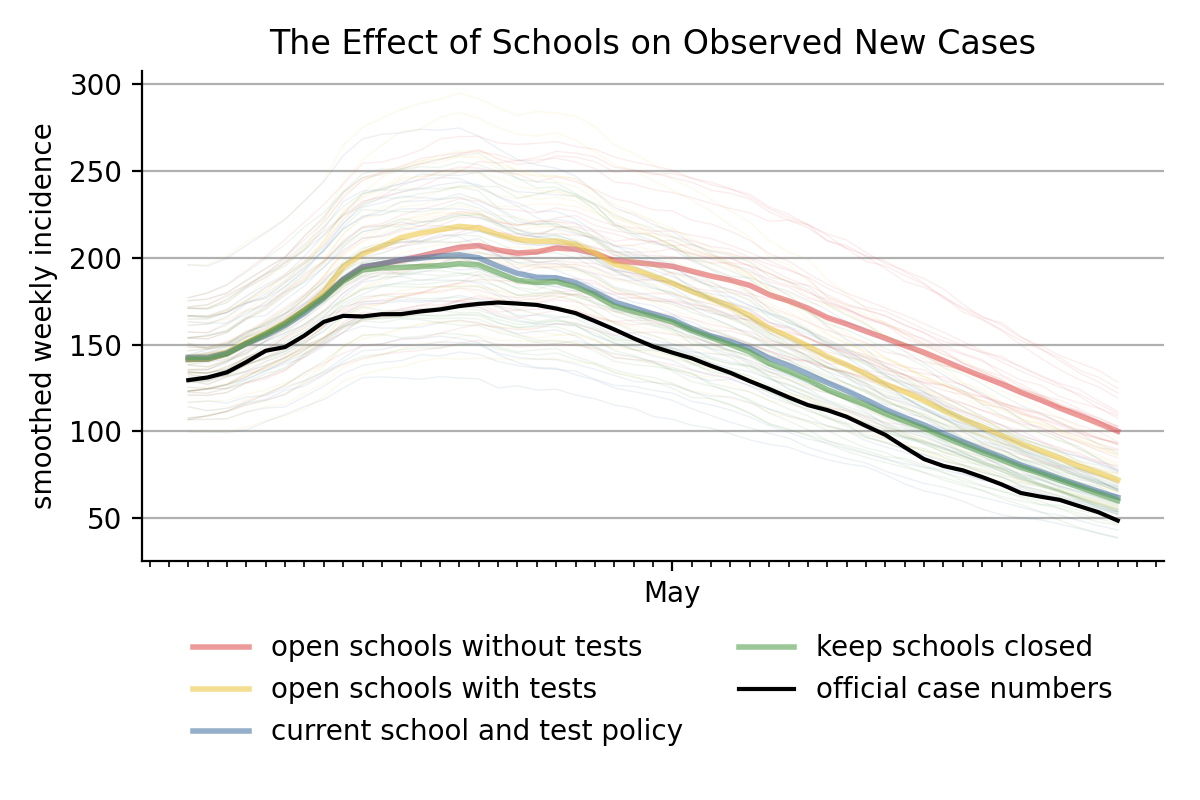
\includegraphics[width=0.9 \textwidth]{../figures/results/figures/comparisons/school_scenarios/full_new_known_case}
    \caption{The Effect of Different School Scenarios on Observed New Cases}
    \label{fig:school_scenarios}
    \figurenotes{\textcolor{red}{\ldots}}
\end{figure}


\FloatBarrier

\begin{tabular}{lr}
\toprule
{} &  predicted total infections among 5-14 year olds from Easter until 2021-05-31 \\
scenario                               &                                                                               \\
\midrule
 educ open after easter  without tests &                                             775324 \\
 educ open after easter  with tests    &                                             604078 \\
 close educ after easter               &                                             469274 \\
 baseline                              &                                             478080 \\
\bottomrule
\end{tabular}
